\documentclass[shortpaper,twoside,web]{ieeecolor}
\usepackage{generic}
\usepackage{cite}
\usepackage{amsmath,amssymb,amsfonts}
\usepackage{algorithmic}
\usepackage{graphicx}
\usepackage{textcomp}
\usepackage{hyperref}
\usepackage[T1]{fontenc}
\def\BibTeX{{\rm B\kern-.05em{\sc i\kern-.025em b}\kern-.08em
    T\kern-.1667em\lower.7ex\hbox{E}\kern-.125emX}}
\newcommand{\tss}[1]{\textsuperscript{#1}}
\newcommand{\tsu}[1]{\textsubscript{#1}}
\newcommand{\td}{\textasciitilde}

\markboth{\journalname, VOL. XX, NO. XX, XXXX 2020}
{Shirazi and Huang: Differential theta-band signatures of seated locomotor perturbations}
\begin{document}
\title{Differential theta-band signatures of the anterior cingulate and motor cortices during seated locomotor perturbations}
\author{Seyed Yahya Shirazi, \IEEEmembership{Student Member, IEEE}, and Helen J. Huang, \IEEEmembership{Member, IEEE}
\thanks{This paragraph of the first footnote will contain the date on 
which you submitted your paper for review. This work was partially supported by the National Institute on Aging of the National Institutes of Health (NIH), under award number R01AG054621.'' }
\thanks{S.Y. Shirazi is with the Mechanical and Aerospace Engineering Department, University of Central Florida (shirazi@ieee.org). }
\thanks{H.J. Huang is with the the Mechanical and Aerospace Engineering Department, and the Disability and Assistive Technology (DAT) Cluster, University of Central Florida (hjhuang@ucf.edu).}
}

\maketitle

\begin{abstract}
Quantifying motor and cortical responses to perturbations during seated locomotor tasks such as recumbent stepping and cycling will expand and improve the understanding of locomotor adaptation processes beyond just perturbed gait. Using a perturbed recumbent stepping protocol, we hypothesized motor errors and anterior cingulate activity would decrease with time, and perturbation timing would influence electrocortical elicitation. Young adults (n=17) completed four 10-minute arms and legs stepping tasks, with perturbations applied at every left or right leg extension-onset or mid-extension. A random no-perturbation “catch” stride occurred in every five perturbed strides. We instructed subjects to follow a visual pacing cue and to step smoothly and quantified temporal and spatial motor errors. We used high-density electroencephalography to estimate sources of electrocortical fluctuations shared among >70\% of subjects. Temporal and spatial errors did not decrease from early to late for either perturbed or catch strides. Interestingly, spatial errors post-perturbation did not return to pre-perturbation levels, suggesting use-dependent learning occurred. Theta (3-7 Hz) synchronization in the anterior cingulate cortex and left and right supplementary motor areas (SMA) emerged near the perturbation event, and extension-onset perturbations elicited greater theta-band power than mid-extension perturbations. Even though motor errors did not adapt, anterior cingulate theta synchronization decreased from early to late perturbed strides, but only during the right-side tasks. Additionally, SMA mainly demonstrated specialized, not contralateral, lateralization. Overall, seated locomotor perturbations produced differential theta-band responses in the anterior cingulate and SMAs, suggesting that tuning perturbation parameters, e.g., timing, can potentially modify electrocortical responses. 
\end{abstract}

\begin{IEEEkeywords}
cortical control, mobile brain-body imaging, motor adaptation, use-dependent learning
\end{IEEEkeywords}

\section{Introduction}
\label{sec:introduction}
\IEEEPARstart{M}{otor} adjustments to perturbations are often short-lived and “wash-out” soon after removing perturbations \cite{Torres-Oviedo2011-tv,Huang2012-dr}. Still, experiencing perturbations enhance the response to the same and even new perturbations and can also modify unperturbed locomotion \cite{Leech2018-sr}. Previous studies supported retained post-perturbation modifications for stroke patients after split-crank cycling and split-belt walking \cite{Alibiglou2011-sc,Maclellan2014-vk}. The split-crank study also suggested exclusive post-perturbation motor patterns after cycling with different crank angles \cite{Alibiglou2011-sc}. These discernible motor modifications indicate that perturbations modify motor responses and that the manipulating perturbation features could modulate motor responses. Determining the extent of motor and cortical modifications to different perturbations during a variety of locomotor tasks, beyond just walking, could greatly improve the understanding of locomotor adaptation processes.

Advancements in brain imaging technologies such as high-density electroencephalography (EEG), functional magnetic resonance imaging, and positron emission tomography have helped researchers identify supra-spinal correlates of locomotion \cite{Gramann2011-yj,Enders2016-id,Hinton2019-gg}. The anterior cingulate cortex theta (3-7 Hz) power increases significantly during double-support in walking and during extension-onset in recumbent stepping \cite{Gramann2011-yj,Bradford2016-kp,Kline2016-ci}. These studies suggest that the anterior cingulate activity may be monitoring more demanding locomotion phases. The supplementary motor area (SMA) has similar theta power fluctuations during walking, cycling, and recumbent stepping \cite{Gramann2011-yj,Jaeger2014-ao,Kline2016-ci}. In general, the SMA and the motor cortex exhibit substantial alpha-beta (8-30 Hz) fluctuations during walking, with decreased alpha-beta power indicating active processing in the motor cortex \cite{Nordin2019-gd}.

The anterior cingulate cortex and SMA also both strongly respond to perturbations during walking and standing. Previous studies on split-belt walking, perturbed beam walking, walking over obstacles, and perturbed stepping reported perturbation-elicited activity of anterior cingulate, SMA, or in both areas \cite{Haefeli2011-ym,Bulea2015-dv,Marchal-Crespo2017-fn,Peterson2018-ht,Hinton2019-gg,Nordin2019-ar}. The anterior cingulate cortex (or the equivalent mid-prefrontal cortex in the EEG channel studies) activity is often associated with error monitoring or motor learning, while SMA activity is associated with sensorimotor integration \cite{Ridderinkhof2004-jx,Galea2011-jf,Peterson2018-ht}. If the anterior cingulate cortex has an error monitoring function, we expect that the activity would scale with the error size \cite{Arrighi2016-yb}. If the anterior cingulate has a role in motor learning, we expect the activity would decrease with more perturbation experience. Previous studies on walking over obstacles and perturbed standing did not observe decreased anterior cingulate activity with more experience \cite{Haefeli2011-ym,Mierau2015-fd}. On the other hand, a recent study reported scaling of central midline EEG signals at the Cz electrode with balance performance during a perturbed standing task \cite{Payne2020-hl}. However, all three studies had insufficient spatial resolution to determine confidently whether the electrocortical dynamics were from a single functional cortical area.

The purpose of this study was to determine the electrocortical signatures of motor responses to perturbations during a seated locomotor task. To our knowledge, there are no studies that have investigated locomotor adaptation and their electrocortical correlates during a seated locomotor task. Adding perturbations during seated locomotor tasks such as recumbent stepping, which likely shares neural control with walking \cite{Stoloff2007-da,Zehr2007-ww} could provide an alternative option for gait rehabilitation since subjects do not need to maintain their balance. Using our motorized recumbent stepper \cite{Huang2009-of}, we applied discrete mechanical perturbations during each stride and also had intermittent no-perturbation "catch" strides. The catch strides could probe whether subjects were updating anticipatory motor control strategies. We used high-density EEG, independent component analysis (ICA), and a source estimation technique to identify activity of cortical sources during this experiment.

We had two hypotheses related to adaptation, a third hypothesis about perturbation timing, and a fourth hypothesis about motor cortex lateralization. The first adaptation hypothesis was that perturbations would initially create motor errors and increase anterior cingulate theta power near the perturbation event. As subjects gained more experience with perturbations, motor errors, and anterior cingulate theta power would decrease. The second adaptation hypothesis was that motor errors during the no-perturbation catch strides would increase the more subjects expected to encounter perturbations and that anterior cingulate spectral fluctuations would decrease in the later catches. We also hypothesized that perturbations during the middle of leg extension, when the limbs were moving the fastest, would produce more significant errors and anterior cingulate theta power than perturbations at the beginning of leg extension. We also expected to identify left and right motor cortices based on recumbent stepping studies \cite{Jaeger2014-ao,Kline2016-ci}. As such, we planned to compare the time-frequency spectral plots of the left and right motor cortices in response to the perturbations to explore the lateralized cortical activity.

\begin{figure}[!t]
\centerline{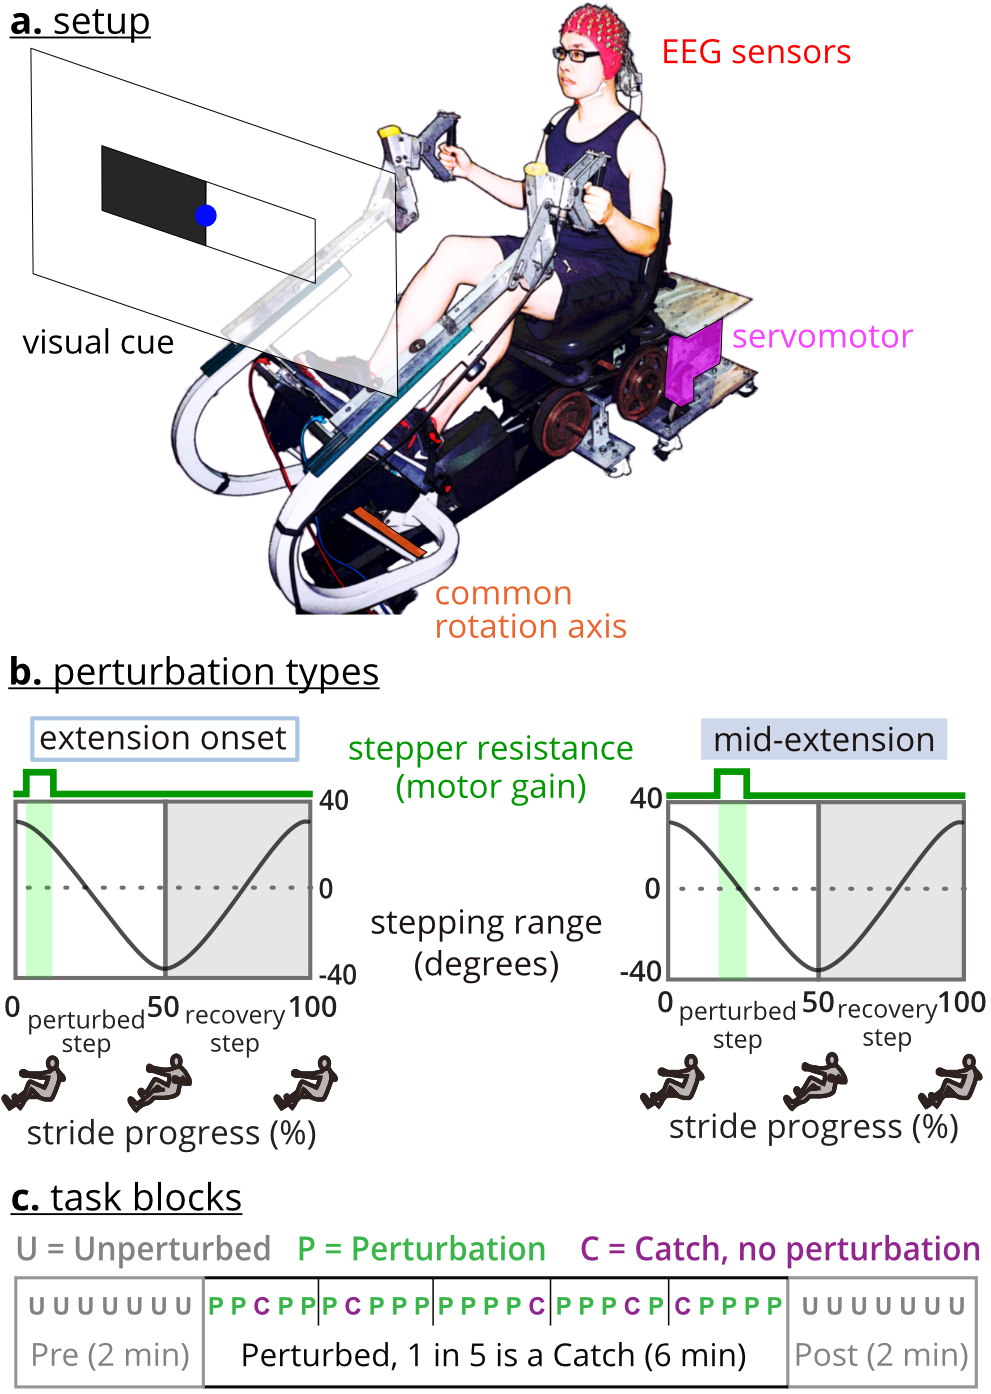
\includegraphics{figures/01_device-protocol_errorMetric.jpg}}
\caption{\textbf{Recumbent stepper and perturbations.} \textbf{a.} The recumbent stepper is a one-degree-of-freedom arm-leg exercise device. \textbf{b.} Perturbations were applied either at the extension-onset or mid-extension of the targeted leg. Perturbations were in the form of increased resistance in stepping for 200 milliseconds. \textbf{c.} The experiment included four tasks. Each task included three ordered blocks, pre, perturbed stepping, and post. The perturbed stepping block also included random no-perturbation catch strides every five perturbed strides.}
\label{fig1}
\end{figure}

\section{Methods}
\label{sec:methods}
Subjects (n=17, 11 females, age 25 ± 4.9 years) performed perturbed arm-leg stepping on a one degree-of-freedom recumbent stepper integrated with a servomotor. The stepper’s pedals and handles were mechanically and contralaterally coupled, such that the left handle and the right pedal extend together, out of phase with the right handle and left pedal that extend together. This coupling enabled subjects to use any combination of their arms and legs to drive the stepper.

\subsection{Experiment procedure and motor errors}
The Institutional Review Board of the University of Central Florida approved the protocol and consent form, and the study was conducted per the principles stated in the Declaration of Helsinki. All subjects gave their written informed consent before starting the experiment. Subjects were all right-handed, based on the hand they would use to pick an object from the floor. Subjects self-reported no prior neurological or musculoskletal problems in the past two years before the data collection date. All subjects also met the inclusion criteria for the short performance battery, Berg balance scale examination, and mini mental-state examination.

After placing the EEG cap on the subject’s head according to the BioSemi guidelines, we digitized the electrodes and fiducial locations using an infrared 3D scanner (Structure Sensor, Occipital Inc., Boulder, CO). We ensured that the resistance between the scalp and each electrode was <20 Ohms, indicating good contact between the electrodes and the scalp. We recorded EEG using a 128-electrode EEG system (ActiveTwo, BioSemi B.V., Amsterdam, the Netherlands) at a sampling frequency of 512 Hz and triggered to start and stop based on a synchronization signal sent from the stepper. We controlled for EEG cable sway artifact by restricting cable movement using a cable holder behind the subject’s head and instructing subjects to keep their head steady \cite{Symeonidou2018-ge}. We strapped subjects' feet to the pedals after they sat on the stepper seat. We also adjusted the handles to ensure that subjects were comfortable using the handles to drive the stepper.

The stepper’s servomotor perturbed the stepping motion with brief 200 ms increases in resistance at either the onset or middle of extension of the target (left or right) leg during the stepping stride (Figure 1). The increased resistance magnitude during a perturbation required 3x the torque to maintain the stepping pace of 60 steps per minute. In total, there were four perturbation types (left/right leg * mid-extension/extension onset). We provided subjects with a visual pacing cue equal to 60 steps per minute (=30 strides per minute) to maintain the same stepping speed during the tasks.
\begin{figure}[!t]
\centerline{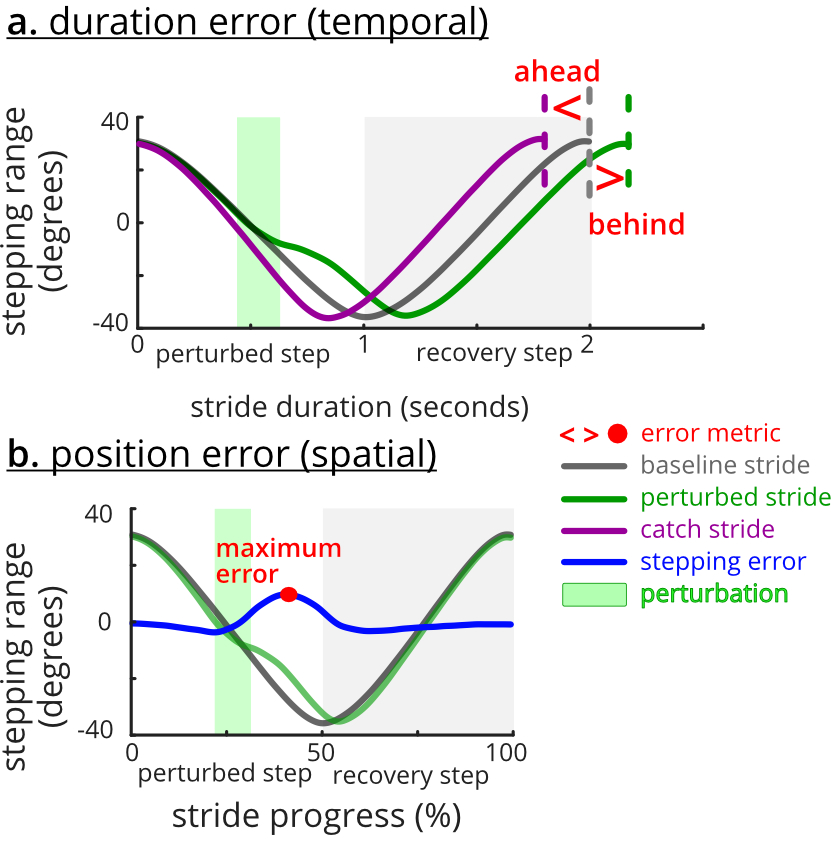
\includegraphics{figures/02_error_metrics.jpg}}
\caption{\textbf{Motor error metrics.} Subjects were instructed to match the pace and step smoothly. \textbf{a.} The stepping duration (i.e., temporal) error is the difference between each stride duration and the two-second pacing cue. \textbf{b.} The stepping position (i.e., spatial) error is the maximum difference between the time-normalized stepper position during each stride and the averaged pre-perturbation stepping profile.}
\label{fig2}
\end{figure}
\subsubsection{Data collection}
The data collection began with two minutes of quiet sitting, during which the visual pacing cues were shown as EEG was recorded. After completing this quiet sitting portion, subjects completed four 10-minute perturbed stepping \textit{\underline{tasks}} in a pseudo-randomized order. Each task only included one perturbation type. For each task, there were three ordered \textit{\underline{blocks}}: 1) \textbf{pre}: two minutes of unperturbed stepping, 2)  \textbf{perturbed stepping}: six minutes of a single perturbation timing, and 3)  \textbf{post}: two minutes of unperturbed stepping (Figure 1). There were no pauses between blocks. In addition to perturbed strides, the perturbed stepping block included random one-in-five “catch” strides where no perturbation was applied. In this paper, we use pre and pre-perturbation and post and post-perturbation interchangeably. There was two minutes of quiet sitting at the end of the data collection.

Before starting each task, we instructed subjects to \textbf{A)} step smoothly as if they were walking, \textbf{B)} use both their arms and legs to drive the stepping motion, and \textbf{C)} follow the visual pacing cues that were projected in front of them (Figure 1). We did not instruct subjects on how to follow the pacing cues as there are several options, such as having a leg be at full extension when the rectangle on the same side as the leg was black. Subjects also received no explicit feedback on whether they were stepping faster or slower than the pacing cue. Subjects were given at least two minutes of practice with the visual pacing cues before starting the data collection.

\subsubsection{Stride events}
After importing stepping data into MATLAB (R2018b, MathWorks Inc, Natick, MA), we separated each task into blocks and strides. We defined the strides as the time from one extension-onset of the perturbed leg to the next extension-onset of the perturbed leg. We excluded any incomplete strides. For each stride, we identified the following \textit{\underline{events}}: perturbed-step extension onset, perturbation (start time), recovery-step extension onset, and the end of the stride. We artificially added perturbation events to the unperturbed strides (i.e., pre, post, and catch strides), equal to the average latency of the perturbation events.

\subsubsection{Motor errors}
We quantified two motor error metrics, one temporal and one spatial, from the stepping kinematics (Figure 2). In our tasks, subjects should have completed a stride in two seconds based on the 60 steps-per-minute visual pacing cues. Therefore, we defined temporal error as the stepping duration error, which was the difference between each stride duration and the two seconds. Because we instructed subjects to step smoothly, we expected the stepping profiles to be smooth and rhythmic during the pre-perturbation block. Therefore, we defined spatial error as a stepping position error, which was the maximum difference between the time-normalized stepper position profile during each stride and the averaged pre-perturbation stepping profile. We used the servomotor position data to quantify the angular stepping position around the stepper's common rotating axis (Figure 1).

\subsection{EEG processing}
EEG data were analyzed in the MATLAB environment (R2018b, MathWorks Inc, Natick, MA) using a customized pipeline based on EEGLAB (version 2019.0) functions \cite{Delorme2004-yy} (Figure 3). We used a high-pass filter at 1 Hz and a 60 Hz line-noise filter (CleanLine) to minimally clean the raw data \cite{Mullen2012-rh,Winkler2015-br}. We imported stride events from the synchronized stepping data and concatenated data from all trials into a single file. Afterward, we used the template correlation rejection method to identify and exclude channels that contained high locomotor-like artifacts \cite{Oliveira2017-pk}.

\begin{figure*}[!ht]
\centerline{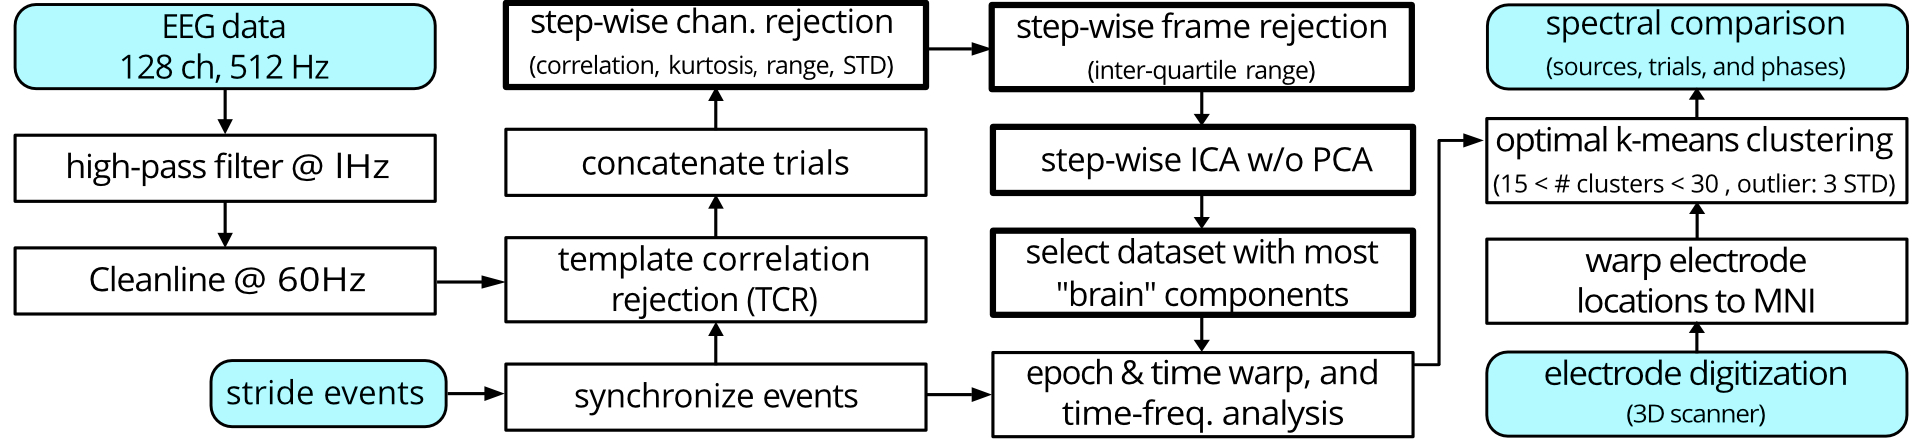
\includegraphics{figures/03_EEG workflow.jpg}}
\caption{\textbf{EEG post-processing workflow with a novel step-wise algorithmic parameter sweeping noise rejection process.} Shaded blocks indicate inputs or outputs. Thick lined blocks highlight the novel step-wise rejection approach.}
\label{fig3}
\end{figure*}

We developed and used a novel step-wise channel and frame rejection algorithm to reject channels and data frames that still contained considerable noise (Figure 3). We removed the researcher's need to set single thresholds for the channel and frame rejection steps. Instead, the step-wise algorithm identified a suite of thresholds, from lenient to conservative, that created 32 separate datasets with different rejection levels for each participant (8 steps for channel rejection * 4 steps for data-frame rejection = 32 datasets). Channel rejection metrics were the signal range, standard deviation, kurtosis, and correlation to the other channels. Frame rejection involved finding periods of the EEG data with a significantly higher signal variability than the overall median of signal variability. While the number of the rejected channels and frames varied for each participant and increment, we set the rejection thresholds such that the most conservative increment always retained > 85 channels and > 80\% of data.

We used ICA, the dipolar source estimation technique (DIPFIT), and a multi-variate source classifier (ICLabel) on each step-wise dataset to identify and locate the sources that contributed to the EEG signals. We specifically used the adaptive mixture independent component analysis (AMICA) to separate the EEG into temporally independent components \cite{Palmer2008-jx}. To select the best increment from the 32 step-wise datasets, we first estimated the source locations for each dataset's independent components using EEGLAB’s DIPFIT version 3.0. We then excluded any source located outside the brain or with the residual variance > 15\%. We then used EEGLAB’s ICLabel toolbox to classify the source types as “brain” or “non-brain” \cite{Pion-Tonachini2017-ez} and selected the step-wise dataset with the topmost “brain” sources as the representative dataset for each subject. We visually checked the results of the ICLabel for the selected dataset to confirm the classification of the sources as “brain” (or “non-brain”).

We then clustered the sources across all subjects based on the source location, power spectrum, and scalp map. We divided the power spectrum and scalp map into ten bins. The binned power spectrum was from 3 to 25 Hz. The Laplacian of the scalp map was used for clustering \cite{Hjorth1975-ea}. We developed and used a novel optimal k-means approach to determine the number of clusters from a range of possible numbers of clusters provided to the algorithm (here, from 15 to 30 clusters). The optimal k-means approach uses MATLAB’s “evalcluster” function to find the specific number of clusters that maximize the similarity of the sources within each cluster. We kept and analyzed only the clusters that contained components from more than 70\% of the subjects. If a subject had multiple sources in a cluster, we only kept the source with the largest the channel data variance. We identified Brodmann Areas and cortical cortices of the sources and cluster centroids using Talairach coordinates and \href{http://talairach.org/}{talairach.org} \cite{Lancaster2000-aj,Shirazi2019-im}.

We computed the time-frequency spectral power of each source in the cluster across the stride epochs, known as event-related spectral perturbations (ERSP) \cite{Makeig1993-jx}. For testing hypotheses 1, 2, and 4, each epoch was from the start to the end of a stride. For hypothesis 3, we only looked at epochs from –400 ms to +400 ms of the perturbation event. We extended the epochs by 700 milliseconds to avoid possible edge effects. Next, we baseline-normalized the spectral power based on the pre-perturbation block's average spectral power and computed the ensembled average ERSPs across subjects. We determined the significant event-related synchronization and event-related desynchronization across the ERSPs using EEGLAB’s bootstrapping method with alpha set at 0.05 \cite{Pfurtscheller1999-oi}. We only show significant synchronizations and desynchronizations in the ERSP images.

\begin{figure*}[!ht]
\centerline{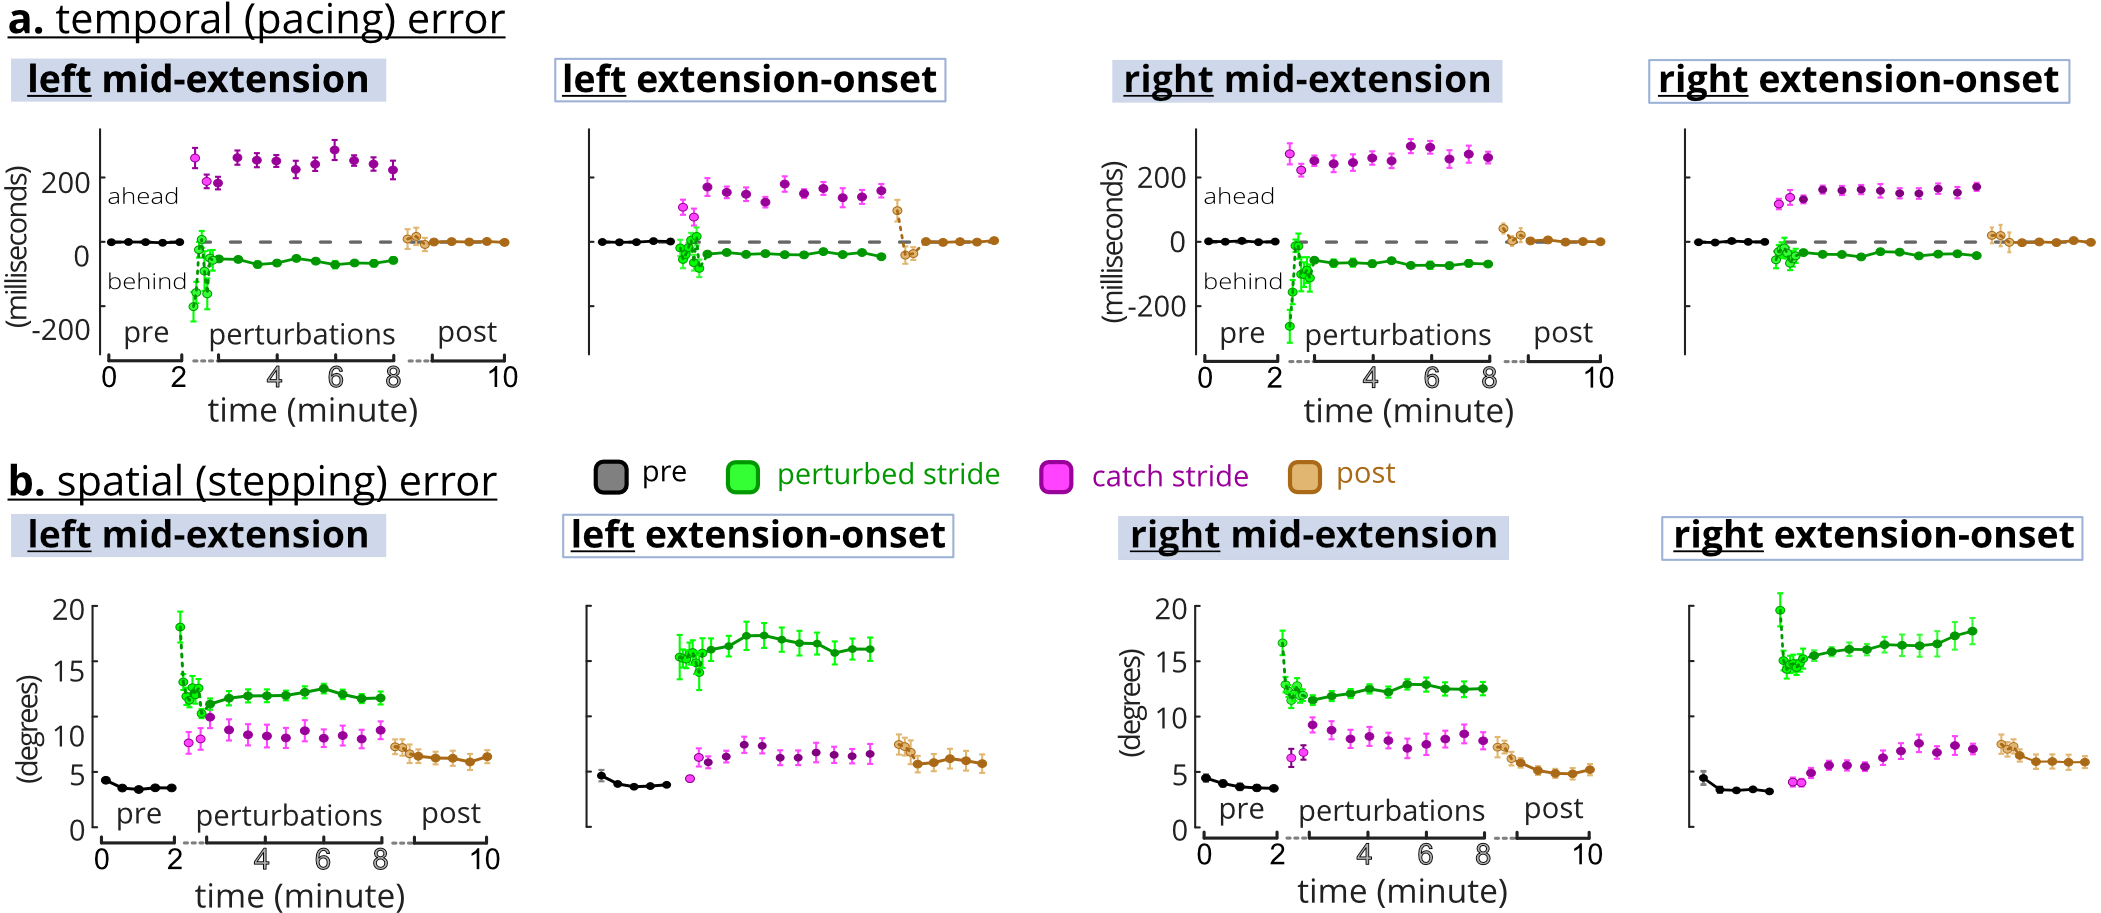
\includegraphics{figures/04_error-result-r2.jpg}}
\caption{\textbf{Temporal and spatial errors during perturbed stepping.} The perturbed stepping block include both perturbed strides (green) and one-in-five random catch strides (purple). Dark circles are the batched average, and the light-colored circles indicate average single strides. Error bars are confidence interval. \textbf{a.} Temporal errors were different between perturbed and catch strides (\td50 ms vs \td200ms) Temporal errors returned to the pre-perturbation levels during the post block. \textbf{b.} Spatial error was greater for the perturbed strides than catch strides. Spatial errors of perturbed strides did not decrease after the first few strides. Post spatial errors did not return to pre-perturbation levels.}
\label{fig4}
\end{figure*}

\subsection{Statistical analysis}
\subsubsection{Tests for hypotheses 1 and 2: adaptation of motor and cortical responses}
We compared motor errors and electrocortical dynamics from early (first 33\% of the strides) to late (last 33\% of the strides) during the perturbed stepping block. We tested motor errors for the perturbed and catch strides separately and used a full factorial repeated-measure analysis of variance (rANOVA) with three factors: 1) \textit{adaptation} with two levels: early and late, 2) \textit{task side} with two levels: left and right, and 3) \textit{perturbation timing} also with two levels: mid-extension and extension-onset. We performed post-hoc Student paired t-tests only if the adaptation had a significant main effect because adaptation was the only factor pertinent to our first two hypotheses. To compare the electrocortical responses between early and late perturbed strides and early and late catch strides, we computed the spectral fluctuations and averaged the spectral powers to derive the theta-band (3-7 Hz) ERSP waveform \cite{Pfurtscheller1999-oi,Wagner2016-nx}. We compared the early and late theta-band average ERSP waveforms using bootstrapped paired t-tests with EEGLAB’s “statcond” function. We also determined meaningful spectral-power increases or decreases of the theta-band by determining when the power confidence interval was greater or less than zero. We did not include other frequency bands in our analysis because our preliminary results showed that the main spectral fluctuations were limited to theta. The significance level for all statistical tests was 0.05.

\subsubsection{Tests for hypothesis 3: effect of perturbation timing}
We included all perturbed strides to quantify possible motor and electrocortical differences between perturbation timings, i.e., mid-extension and extension onset. For each motor error, we used a full factorial rANOVA with two factors: 1) \textit{perturbation timing} with two levels: mid-extension and extension-onset, and 2) \textit{task side} also with two levels: left and right. We only performed a post-hoc Student paired t-test between the same side tasks if there was a significant perturbation timing effect. We constructed spectral fluctuations for all perturbed strides from –400 ms to 400 ms of the perturbation event for the electrocortical responses and compared left-side tasks (i.e., mid-extension and extension-onset) and right-side tasks separately. Similar to the tests for hypotheses 1 and 2, we used bootstrapped paired t-tests for comparing the theta-band average ERSP between the tasks and determined meaningful spectral-power increases or decreases when the power confidence interval cleared zero. The significant level of all statistical tests was 0.05.

\subsubsection{Tests for hypothesis 4, motor cortex lateralization}
We compared the spectral fluctuations of the motor cortex clusters during the left-side and right-side tasks. All perturbed strides and catch strides were included in this analysis. We were specifically interested in contralateral or specialized lateralization. Contralateral limb movements elicit contralateral lateralization in the motor cortex. Specialized lateralization is the presence of spectral fluctuations during both contralateral and ipsilateral limb movements.

\section{Results}
\label{sec:methods}
\subsection{Motor error responses and cortical clusters}

Temporal (pacing) errors during perturbed strides were considerably less than the catch strides (Figure 4a). Subjects reduced their temporal errors to \td50ms after only a few perturbed strides, but their errors during the catch strides were \td200 ms. During the post-perturbation block, subjects reduced their temporal errors to nearly zero after only a few strides. The first perturbed strides in mid-extension tasks had higher temporal errors and variation than the first perturbed strides in extension-onset tasks. However, spatial (stepping) errors for the perturbed strides were larger than the catch strides (Figure 4b). After the first few perturbed strides, subjects kept their error steady, \td12 degrees for the mid-extension tasks and \td16 degrees for the extension-onset tasks. Spatial errors for the catch strides in extension-onset tasks started from the pre-perturbation errors at \td5 degrees but was \td10 degrees toward the end of the catch strides. Spatial errors continued from the catch stride errors during post-perturbation and did not wash out (i.e., return to pre levels) after two minutes of stepping.

The optimal k-means identified five clusters with sources from > 70\% of the subjects (Figure 5). From these five clusters, we focused on three clusters located at the anterior cingulate cortex (14 subjects), left SMA (13 subjects), and right SMA (13 subjects). Locations of the clusters were determined by assigning the nearest Brodmann areas to the Talairach coordinates of the cluster centroid \cite{Shirazi2019-im}. As SMA and premotor cortex share Brodmann area 6, we confirmed from a previous fMRI and PET meta-analysis that SMA cluster centroids were indeed in the SMA region, not the premotor \cite{Mayka2006-ye}. The left and right SMA were determined based on the cluster’s centroid location and the location of individual sources. Ten out of the thirteen left SMA and eleven out of thirteen right SMA sources were on the left or right hemispheres.

\begin{figure*}[!ht]
\centerline{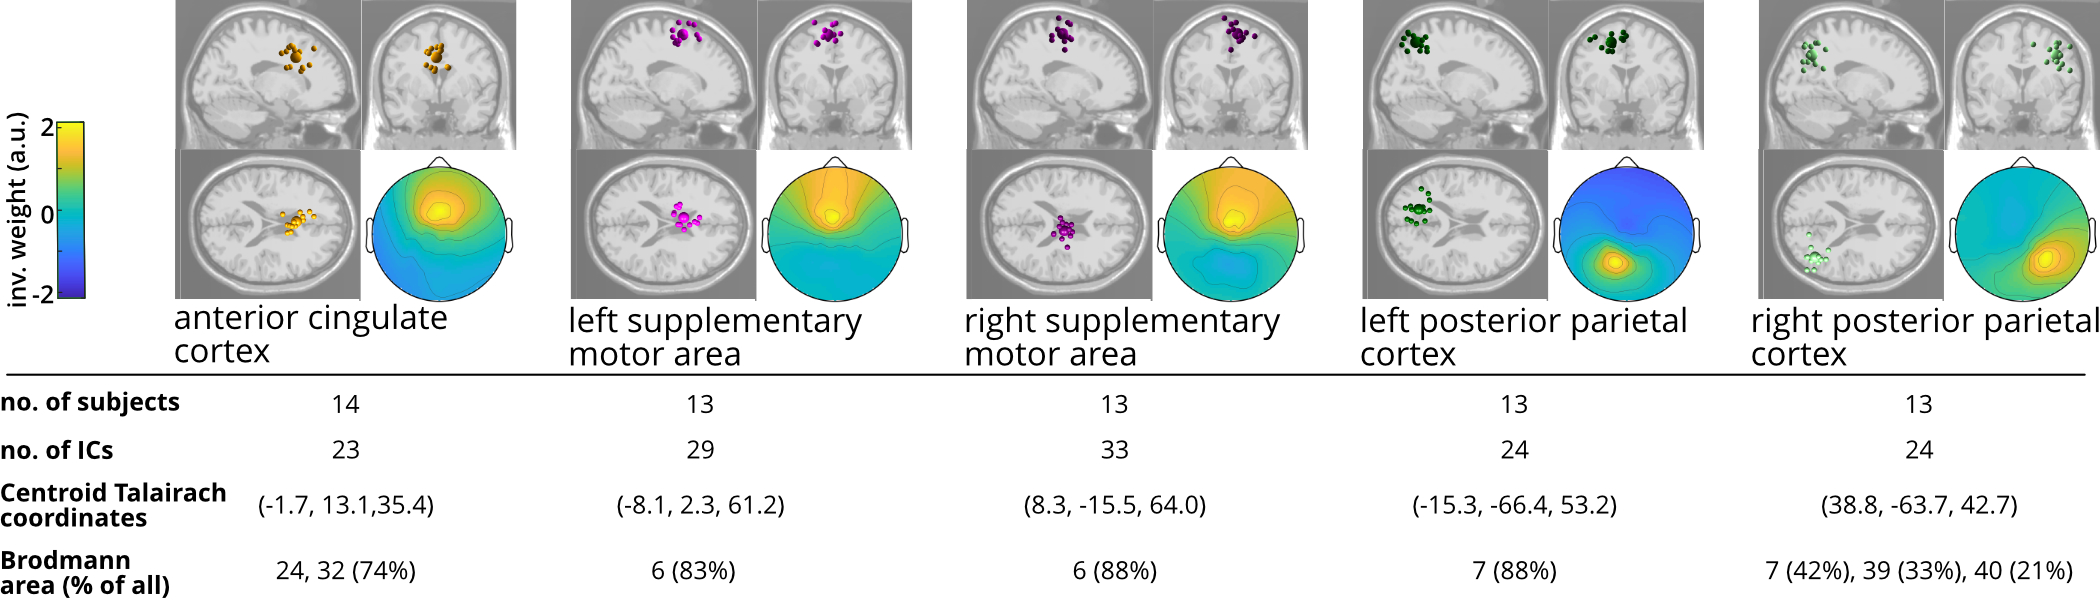
\includegraphics{figures/05_dipole locations_70p.jpg}}
\caption{\textbf{Locations of the electrocortical clusters.} We chose clusters with sources from > 70\% of the subjects. We only selected one source per subject for analysis. The cluster-average scalp projections are ICA inverse weights. a.u.: arbitrary unit}
\label{fig5}
\end{figure*}

\subsection{Anterior cingulate theta-band adaptation occurred without motor error adaptation in perturbed strides}
Motor errors did not decrease from the first (i.e., early) to last (i.e., late) 33\% of the perturbed strides, but there was decreased anterior cingulate theta-band spectral power in the right-side tasks. Neither adaptation nor task side had a significant effect on the perturbed strides (rANOVA, temporal adaptation: F\tsu{(1,16)}=0.74, p=0.789, temporal side: F\tsu{(1,16)}=0.74, p=0.789, spatial adaptation: F\tsu{(1,16)}=2.98, p=0.104, spatial side: F\tsu{(1,16)}=0.71, p=0.413). Mid-extension perturbed strides had significantly greater average temporal errors (71 vs 39 ms) and but smaller spatial errors (12 vs 16 degrees) than the extension-onset catch strides (rANOVA, temporal: F\tsu{(1,16)}=461, p<0.0005, spatial: F\tsu{(1,16)}=30.6, p<0.0005). Perturbations elicited anterior cingulate theta synchronization during all tasks (Figure 6c). Compared to early perturbed strides, theta spectral power decreased during the late right-side perturbed strides. The left-side perturbed strides, however, had similar or even stronger theta synchronization during late strides than the early strides. The anterior cingulate cortex also showed theta desynchronization in the recovery steps (i.e., the unperturbed steps after the perturbed steps), specifically for the early right-side and the late left-side perturbations. The theta-band average ERSP bootstrap t-tests revealed that the spectral power decreased from early to late following the right-side perturbations (Figure 6d). Late desynchronizations during the recovery steps for the left-side perturbations was statistically different from the non-significant spectral fluctuations during early perturbed stepping.
% \begin{figure}[!t]
% \centerline{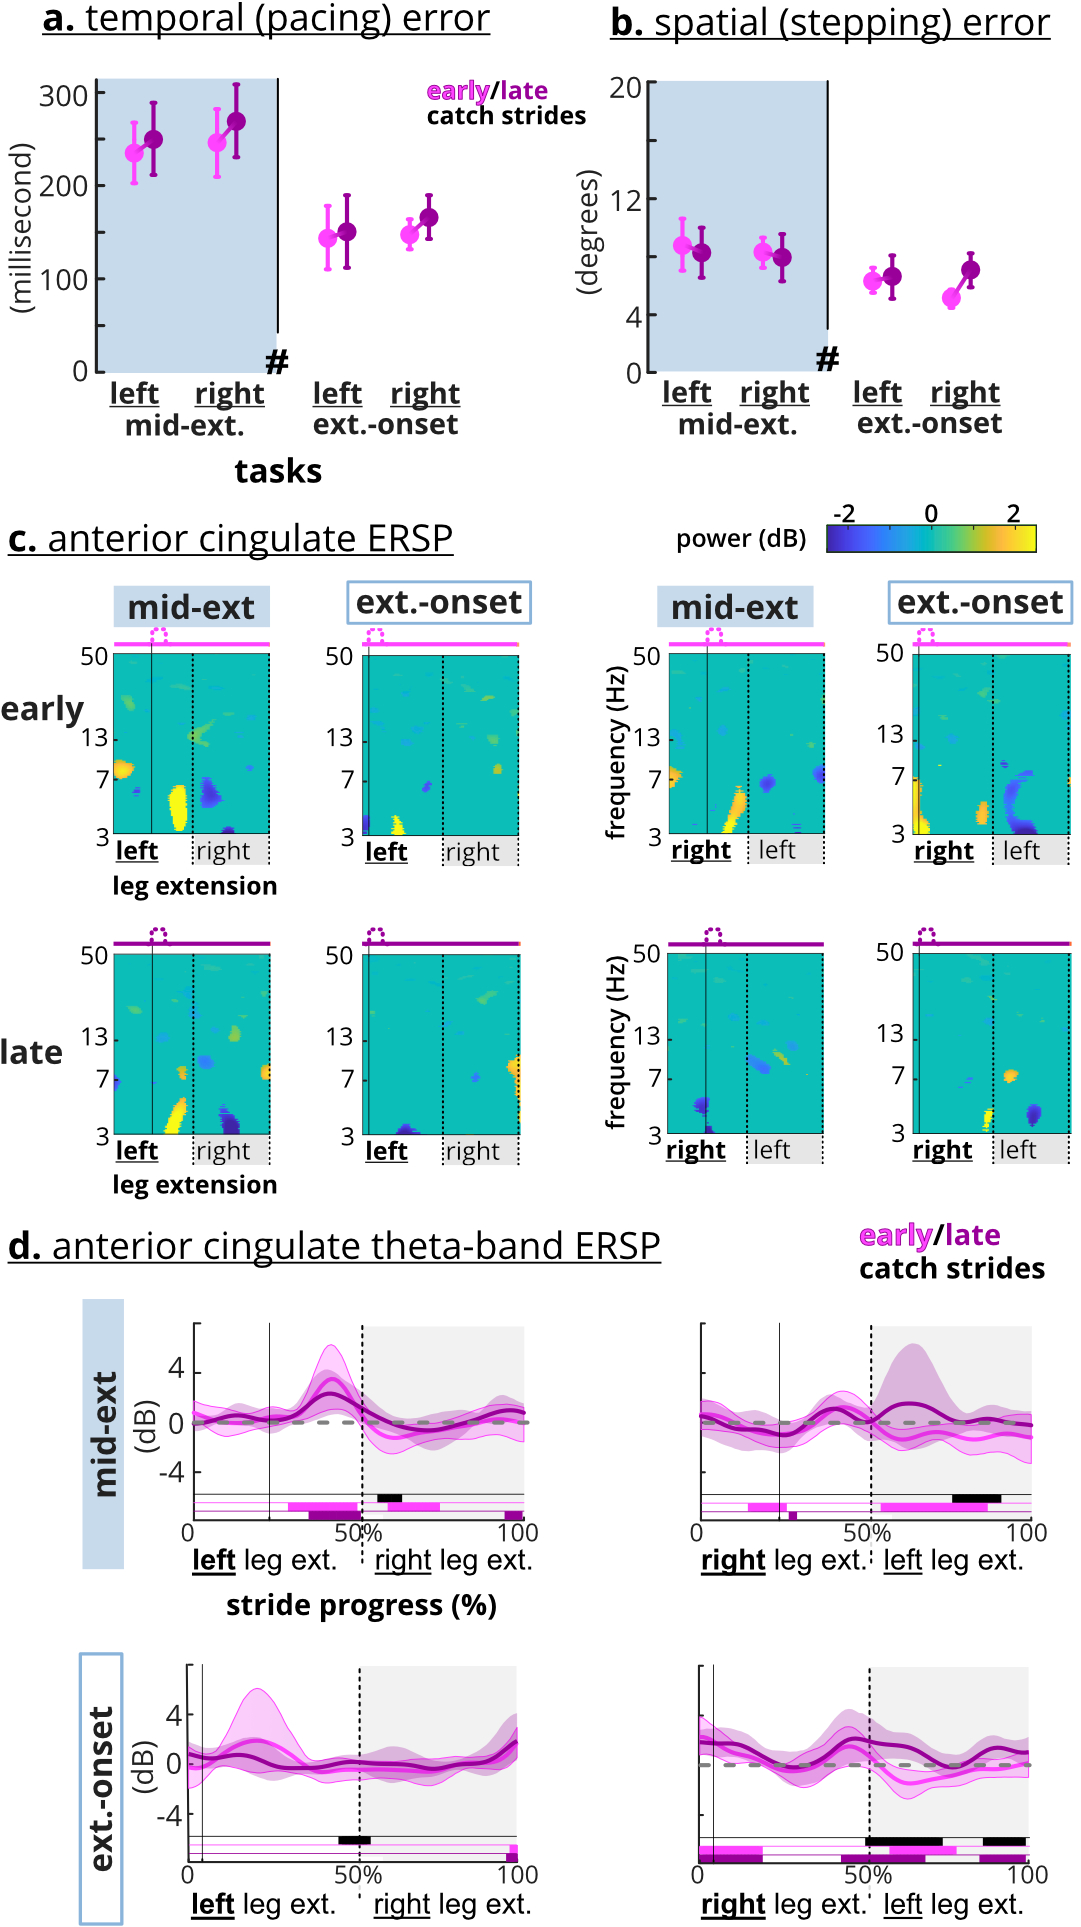
\includegraphics[width=\columnwidth]{figures/hyp2- early late catch.jpg}}
% \caption{\textbf{Catch strides motor errors and anterior cingulate ERSP.} a. and b. Adaptation (early vs. late). There was a significant effect of perturbation timing (indicated by \#). Error bars indicate confidence interval c. Early catches (the narrow solid lines) elicited theta synchronization. d. Late right extension-onset catch strides elicited significantly higher spectral power than early. Shaded areas indicates confidence interval.}
% \label{fig7}
% \end{figure}

\subsection{Anterior cingulate theta-band adaptation occurred without motor error adaptation in catch strides}
Motor errors did not increase from early to late catch strides, but early catch strides still elicited theta synchronization in the anterior cingulate cortex. Similar to the perturbed strides, neither adaptation nor task side had a significant effect on the temporal or spatial motor errors (rANOVA, temporal-adaptation: F\tsu{(1,16)}=3.76, p=0.070, temporal-side: F\tsu{(1,16)}=1.65, p=0.217, spatial-adaptation: F\tsu{(1,16)}=1.43, p=0.25, spatial-side: F\tsu{(1,16)}=0.70, p=0.415) (Figure 6a and b). Mid-extension catch strides had significantly greater average temporal (250 vs 153 ms) and spatial errors (8 vs 6 degrees) than the extension-onset catch strides (rANOVA, temporal: F\tsu{(1,16)}=31.9, p<0.0005, spatial: F\tsu{(1,16)}=24.4, p<0.0005). Early catch steps elicited anterior cingulate theta synchronization (Figure 6e). This synchronization occurred before completion of the catch-step extension for the mid-extension tasks but was near the start of the catch step for just the right extension-onset catch strides. The left mid-extension and right extension-onset elicited theta desynchronization in the recovery steps (Figure 6e and f). Comparing the average theta-band ERSP between early and late catch strides, the most notable difference occurred in right extension-onset, where the recovery steps of the late catch strides elicited significantly greater spectral power than the early catch strides.
\begin{figure*}[!t]
\centerline{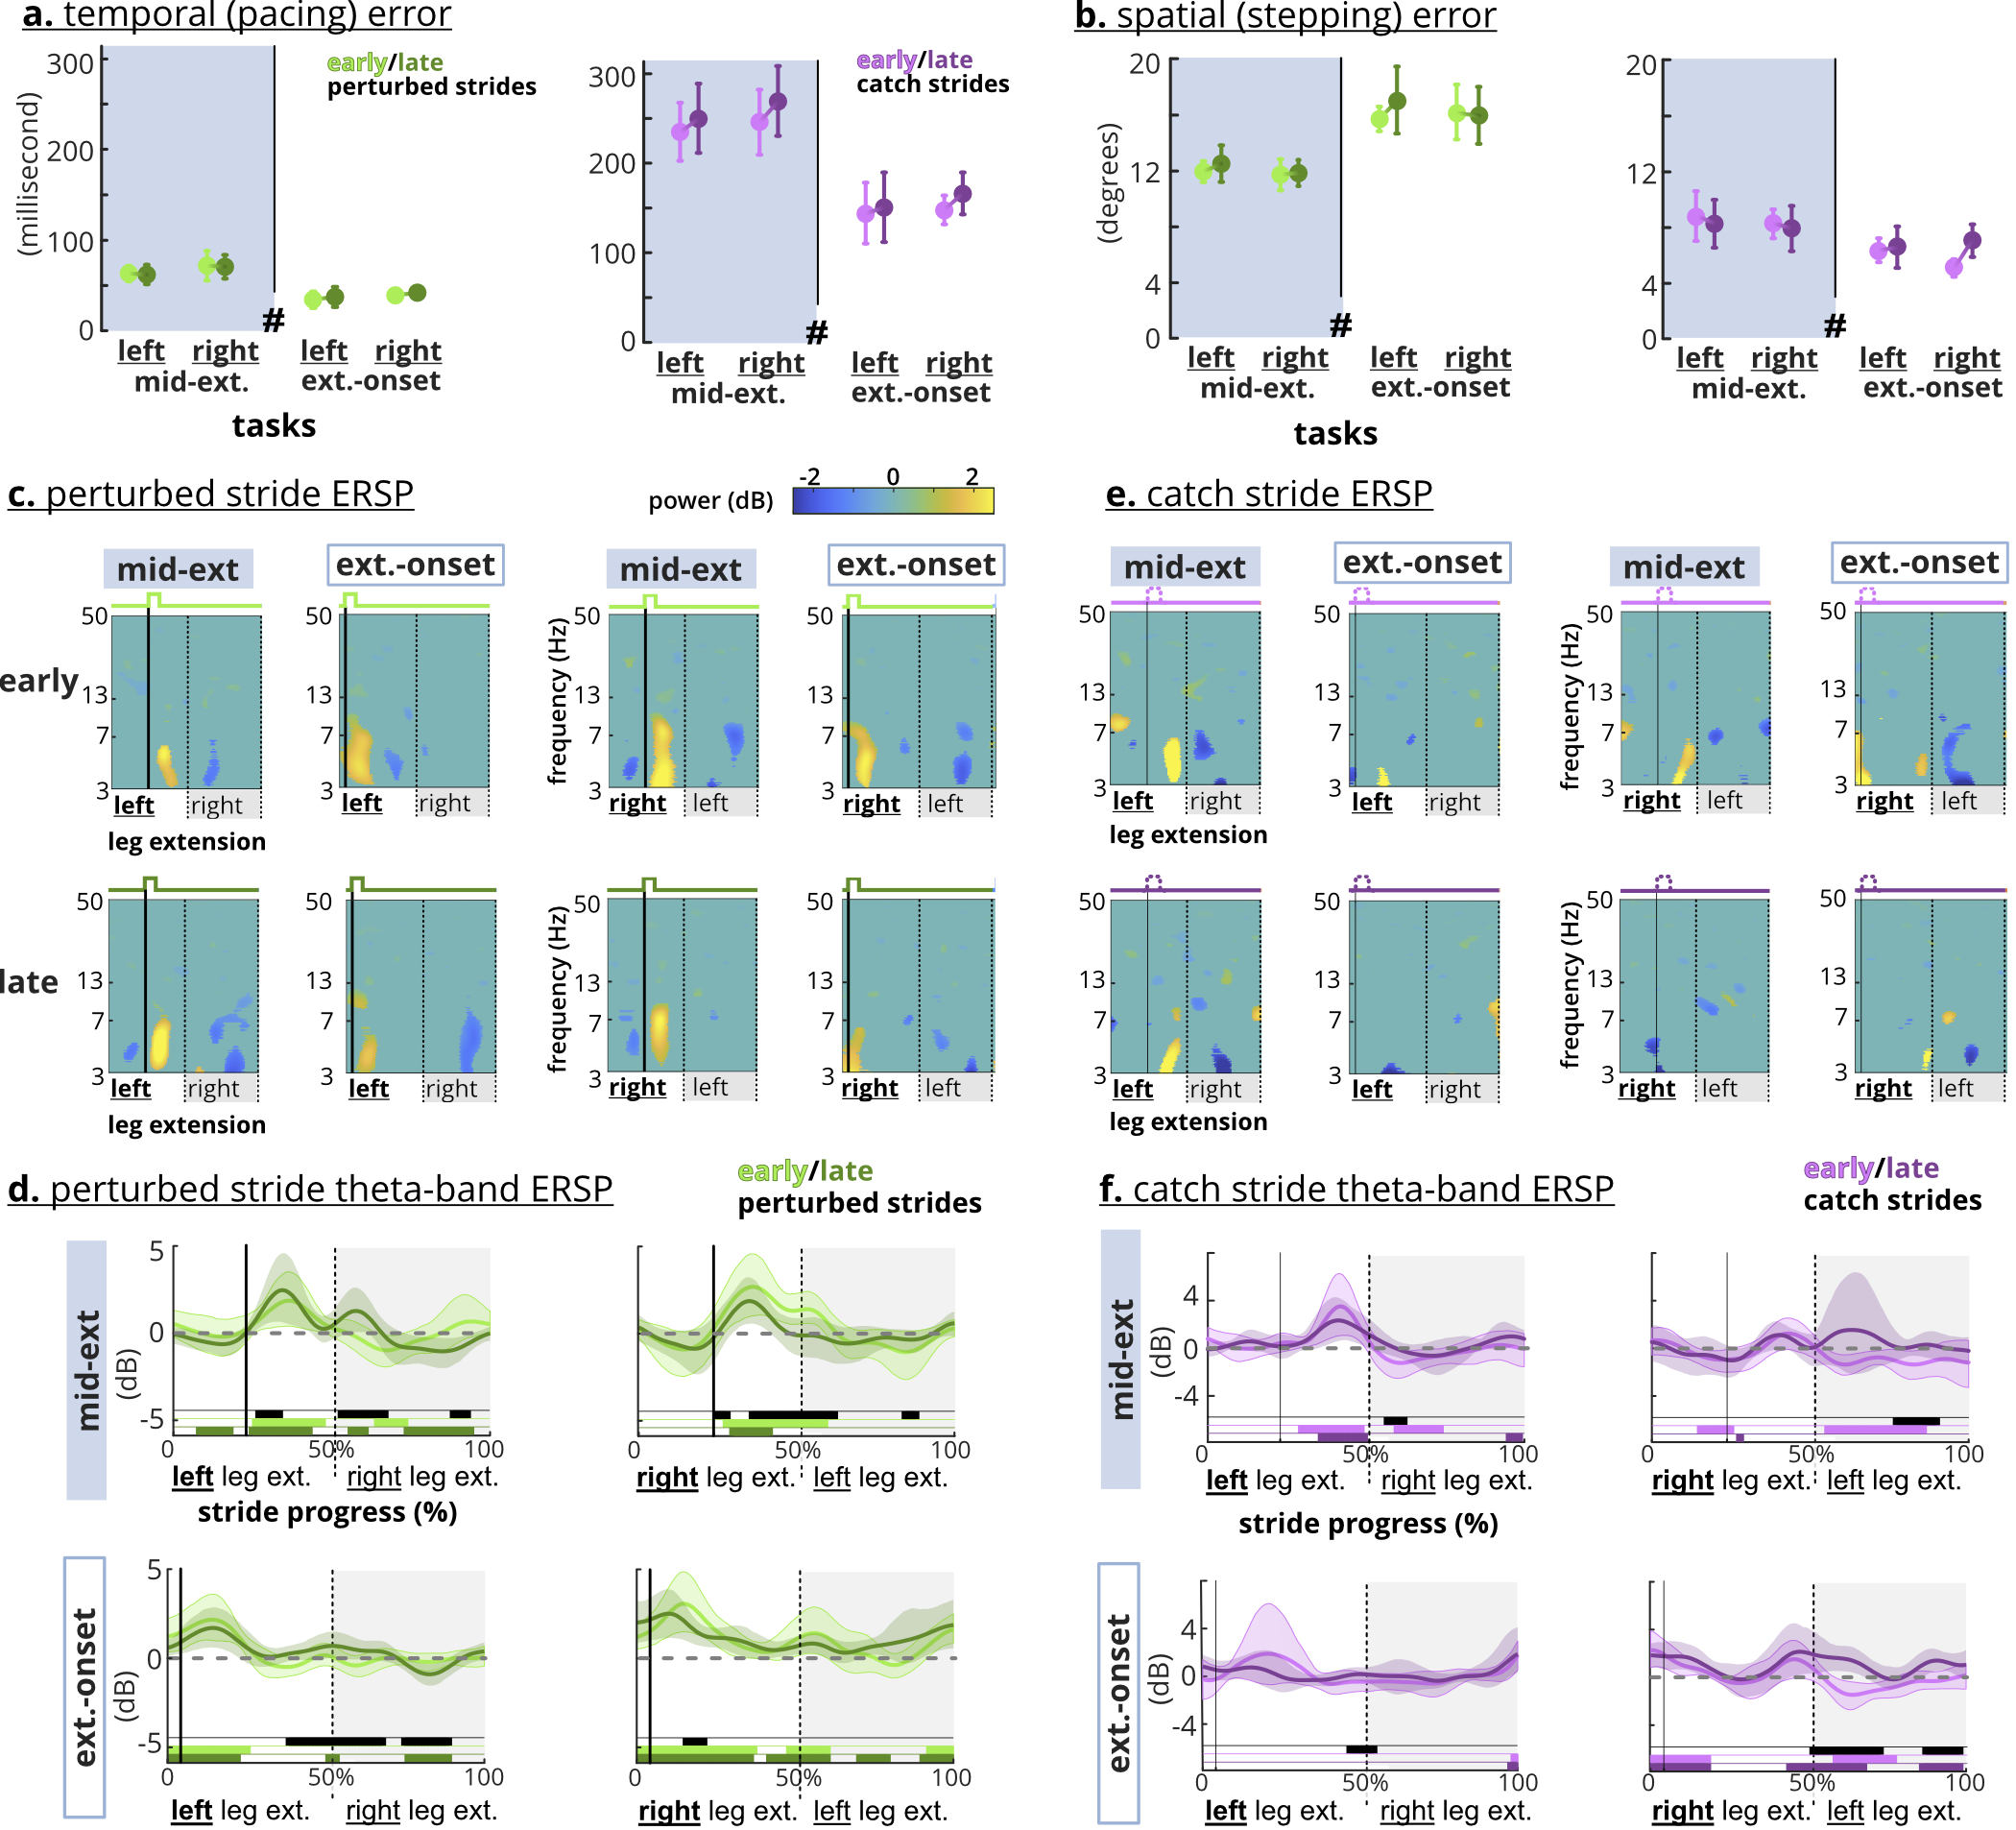
\includegraphics{figures/hyp1and2.jpg}}
\caption{\textbf{Motor errors and anterior cingulate ERSP} \textbf{a.} and \textbf{b.} Adaptation (early vs. late) was not a significant factor for motor errors. \# indicates perturbation timing was a significant factor. Error bars indicate confidence interval (CI) \textbf{c.} Perturbations (i.e., the strong solid lines) elicited theta synchronization in anterior cingulate cortex. Right-side perturbations elicited weaker synchronization during the late perturbed strides. \textbf{d.} Average theta-band ERSP waveform shows increased power after the perturbations across the tasks. Late perturbations elicited less theta-band average power only on the right-side tasks. \textbf{e}. Early catches (narrow solid lines) elicited a theta synchronization in the anterior cingulate cortex. \textbf{f.} Average theta-band ERSP waveform shows late right extension-onset catch strides elicited significantly higher spectral power than the early catch. Shaded areas indicate CI. Black bars indicate significant difference between early and late. Colored bars indicate CI does not overlap with zero.}
\label{fig6}
\end{figure*}

\begin{figure}[!t]
\centerline{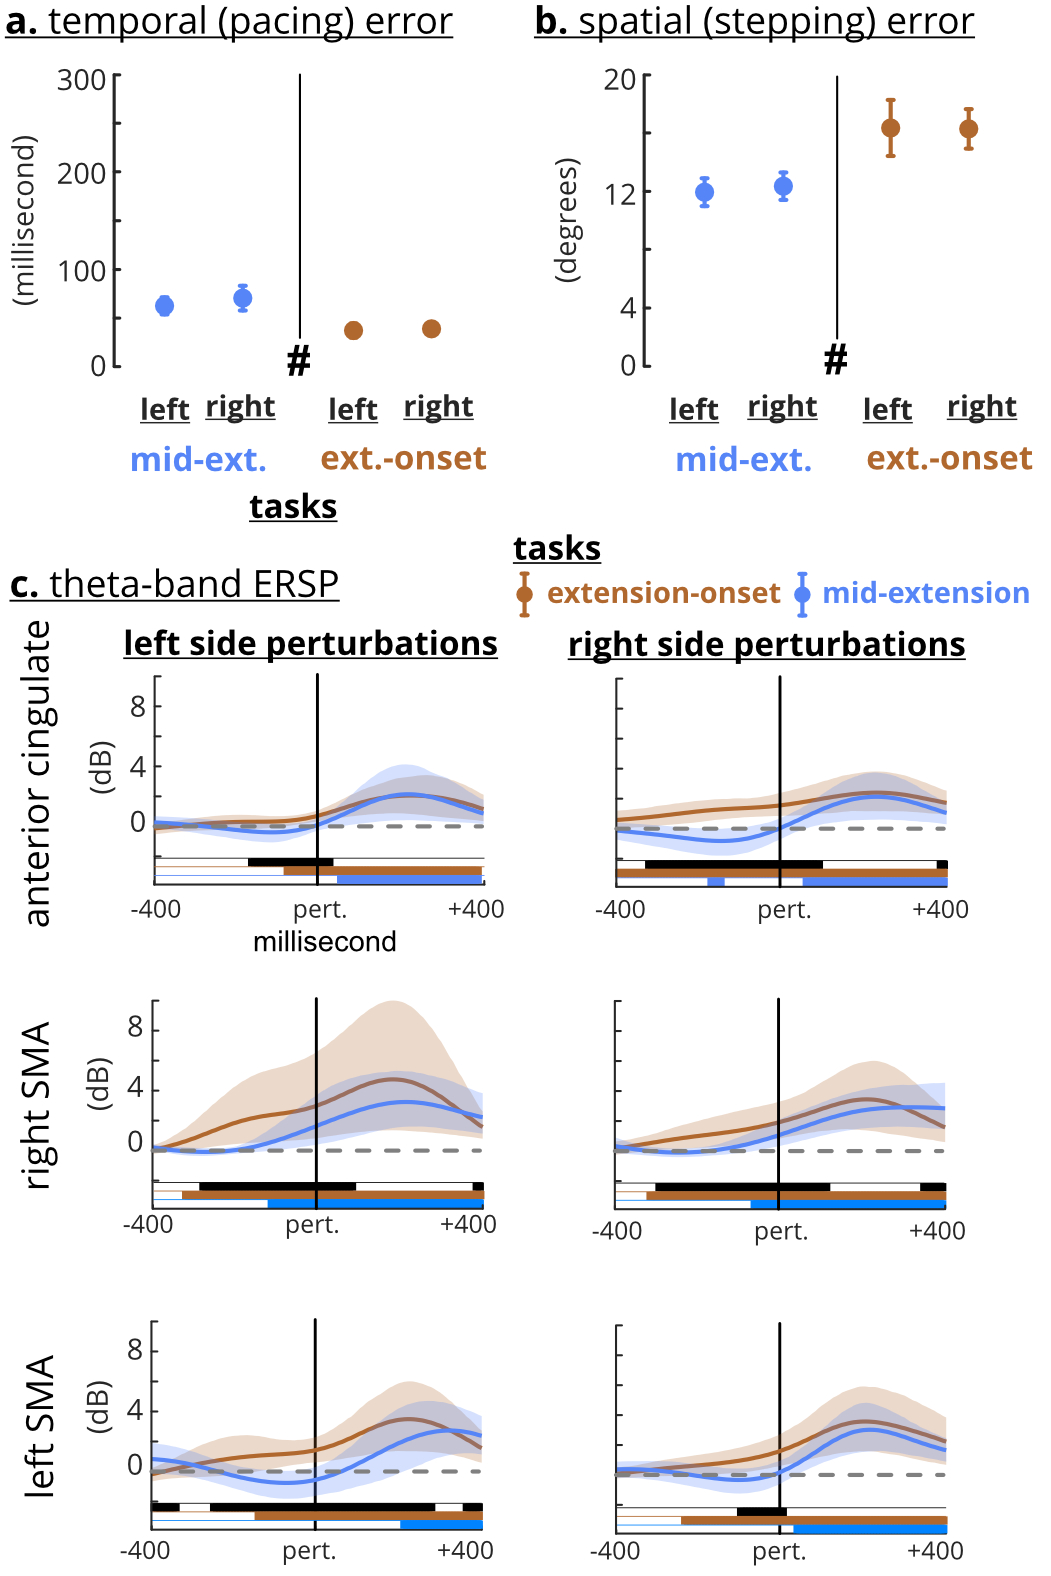
\includegraphics{figures/hyp3 - perturb timing.jpg}}
\caption{\textbf{Motor errors and theta-band ERSP across perturbation timings.} \textbf{a.} and \textbf{b.} Task type (mid-extension vs. extension-onset) was a significant factor for motor errors. Error bars indicate confidence interval. \textbf{c.} Extension-onset perturbations had greater theta-band ERSP before the perturbation event (the solid black line). The theta-band ERSP was not significantly different after the perturbation event, except for the left SMA and left-side tasks. Shaded area indicates confident interval. Black bars indicate significant difference between perturbation timing.Colored bars indicate CI does not overlap with zero.}
\label{fig8}
\end{figure}

\subsection{Perturbations at extension-onset had greater theta-band ERSP in motor cortices than at mid-extension}
Group analyses including all perturbed strides revealed differential motor error and cortical responses based on perturbation timing (Figure 7). Comparing motor errors across all perturbed strides revealed that perturbation timing, and not the task side, was a significant factor (rANOVA, temporal timing: F\tsu{(1,16)}=30.5, p<0.0005, temporal side: F\tsu{(1,16)}=2.24, p=0.15, spatial timing: F\tsu{(1,16)}= 27.5, p<0.0005, spatial side: F\tsu{(1,16)}=0.25, p=0.62) (Figure 7a and b). For each side, temporal error was significantly greater during mid-extension than extension-onset and was smaller during mid-extension than extension onset (post-hoc paired t-test, temporal right: p<0.0005, temporal left: p=0.001, spatial right: p<0.0005, spatial left: p=0.001). The extension-onset perturbations elicited a significant increase in theta-band ERSP before the perturbation event across the anterior cingulate cortex, left SMA, and right SMA (Figure 7c). The increased theta-band ERSP for mid-extension perturbations was delayed until after the perturbation event in the anterior cingulate cortex and left SMA and about -100 ms before the perturbation event in the right SMA. So, significant differences between extension-onset and mid-extension theta-band ERSP diminished shortly after the perturbation event in all cortical clusters. The only exception was the left SMA and left-side tasks where extension-onset had higher theta-band ERSP than mid-extension.

\subsection{Cortical lateralization and specialization}
The left and right SMAs demonstrated both contralateral and task-specific lateralization with respect to lower limb extension (Figure 8). The recovery-step desynchronization during the perturbed strides was most prominent in the right SMA for extension-onset tasks and in the left SMA for the mid-extension tasks, indicating presence of task-specific lateralization (Figure 8a, red rectangles). Mid-extension tasks also involved theta desynchronization before the perturbation event in both left and right SMAs (Figure 8a, red dashed rectangles). Similar recovery-step desynchronization was present in the catch strides but were limited to the ipsilateral SMA of the recovery-step leg during extension-onset tasks and to the right SMA for mid-extension tasks (Figure 8b, black and red rectangles). Strong theta synchronization only occurred in the right SMA for mid-extension catch strides just before the end of the catch step (Figure 8b, red dashed rectangles).

\section{Discussion}
\label{sec:Discussion}

We quantified motor and electrocortical responses to frequent perturbations during seated recumbent stepping to gain insight on the electrocortical dynamics of locomotor adaptation. We did not observe typical motor error adaptation. Temporal errors rapidly reduced and remained at \td50ms of the desired pace during perturbed strides and returned to pre-perturbation levels in the post block. Spatial errors, however, did not adapt (decrease) with more exposure to the perturbations and also did not return to pre-perturbation levels in the post block. The lack of error-based adaptation behavior, small temporal errors, and sustained spatial errors in the post block are indicative of use-dependent learning \cite{Diedrichsen2010-as}. Electrocortical sources at the anterior cingulate cortex and supplementary motor areas (SMA) showed that perturbations elicited theta synchronization, as expected. Despite the lack of motor error adaptation, anterior cingulate theta synchronization decreased during late perturbed strides in the right-side tasks. Interestingly, theta-band ERSP during extension-onset tasks started before the perturbation event, resulting in greater theta synchronization in the anterior cingulate cortex and SMAs preceding the perturbation event compared to mid-extension tasks. Motor cortex lateralization was mostly specialized to the tasks, where theta desynchronization occurred during the recovery-step in the right SMA for extension-onset tasks but in the left SMA for the mid-extension tasks. These results highlight that electrocortical and motor responses are not necessarily coupled and that perturbation features such as perturbation timing could be tuned to elicit greater involvement of specific brain areas.

The perturbed recumbent stepping protocol did not produce the typical error reduction and rapid wash-out associated with motor adaptation, but instead, revealed sustained errors during the post-perturbation block (Figure 4), suggesting use-dependent learning occurred. When perturbations do not directly hinder achieving the task goal, use-dependent learning emerges more than error-based adaptation \cite{Diedrichsen2010-as}. With use-dependent learning, motor behaviors are modified in the direction of perturbation and sustained longer after removing the perturbations. Here, matching the stepping pace with the visual pacing cues was the more explicit task goal. Because subjects matched the pacing cues well with temporal errors of \td50 ms, which might be imperceptible for active control adjustments \cite{Carpenter1999-lb}, the perturbations did not hinder achieving the task goal. For the less explicit goal of stepping smoothly, however, spatial errors were sustained during perturbed strides and did not wash out during the 2-minute post-perturbation block. During split-crank cycling and split-belt walking where changing muscle recruitment was not an explicit task goal, muscular activation patterns were sustained  \cite{Alibiglou2011-sc,Maclellan2014-vk}. More recently, a perturbed walking study using brief treadmill belt accelerations during push-off also reported use-dependent learning and sustained post-perturbation gait modifications \cite{Farrens2020-fb}. Longer-lasting locomotor modifications are desirable for gait rehabilitation and warrant further development of use-dependent learning paradigms.

Perturbations during our seated locomotor task elicited significant anterior cingulate theta synchronization that also decreased with time (i.e. adapted) for right-side perturbations, which provides new insights about the role of the anterior cingulate for error monitoring and motor learning. Previous studies have attributed anterior theta synchronization, or the analogous negative deflection in event-related potentials, to physical loss of balance or presence of a postural threat \cite{Adkin2008-fw,Peterson2018-ht}. Our results demonstrated that even without a potential loss of balance, mechanical perturbations can also elicit anterior cingulate activity during locomotion. We also observed adaptation of anterior cingulate theta synchronization for the right-side tasks, which contrasts previous studies that did not observe changes in the anterior cingulate cortex with adaptation but acknowledged a lack of spatial resolution \cite{Haefeli2011-ym,Mierau2015-fd}. Our approach likely had sufficient resolution \cite{Shirazi2019-im, Shirazi2019-ke}, yet we observed anterior cingulate activity adaptation only in the right-side tasks. Additionally, early catch strides elicited theta synchronization, despite smaller motor errors than the late catch strides. This suggests the anterior cingulate perceived early, but not late, catch strides as errors. Overall, the sustained anterior cingulate theta power across all tasks during perturbed stepping further supports that the anterior cingulate cortex has a role in error-monitoring. However, adaptation of theta-band synchronization during right-side perturbed stepping suggests that the anterior cingulate also has a role in locomotor learning.


\begin{figure}[!t]
\centerline{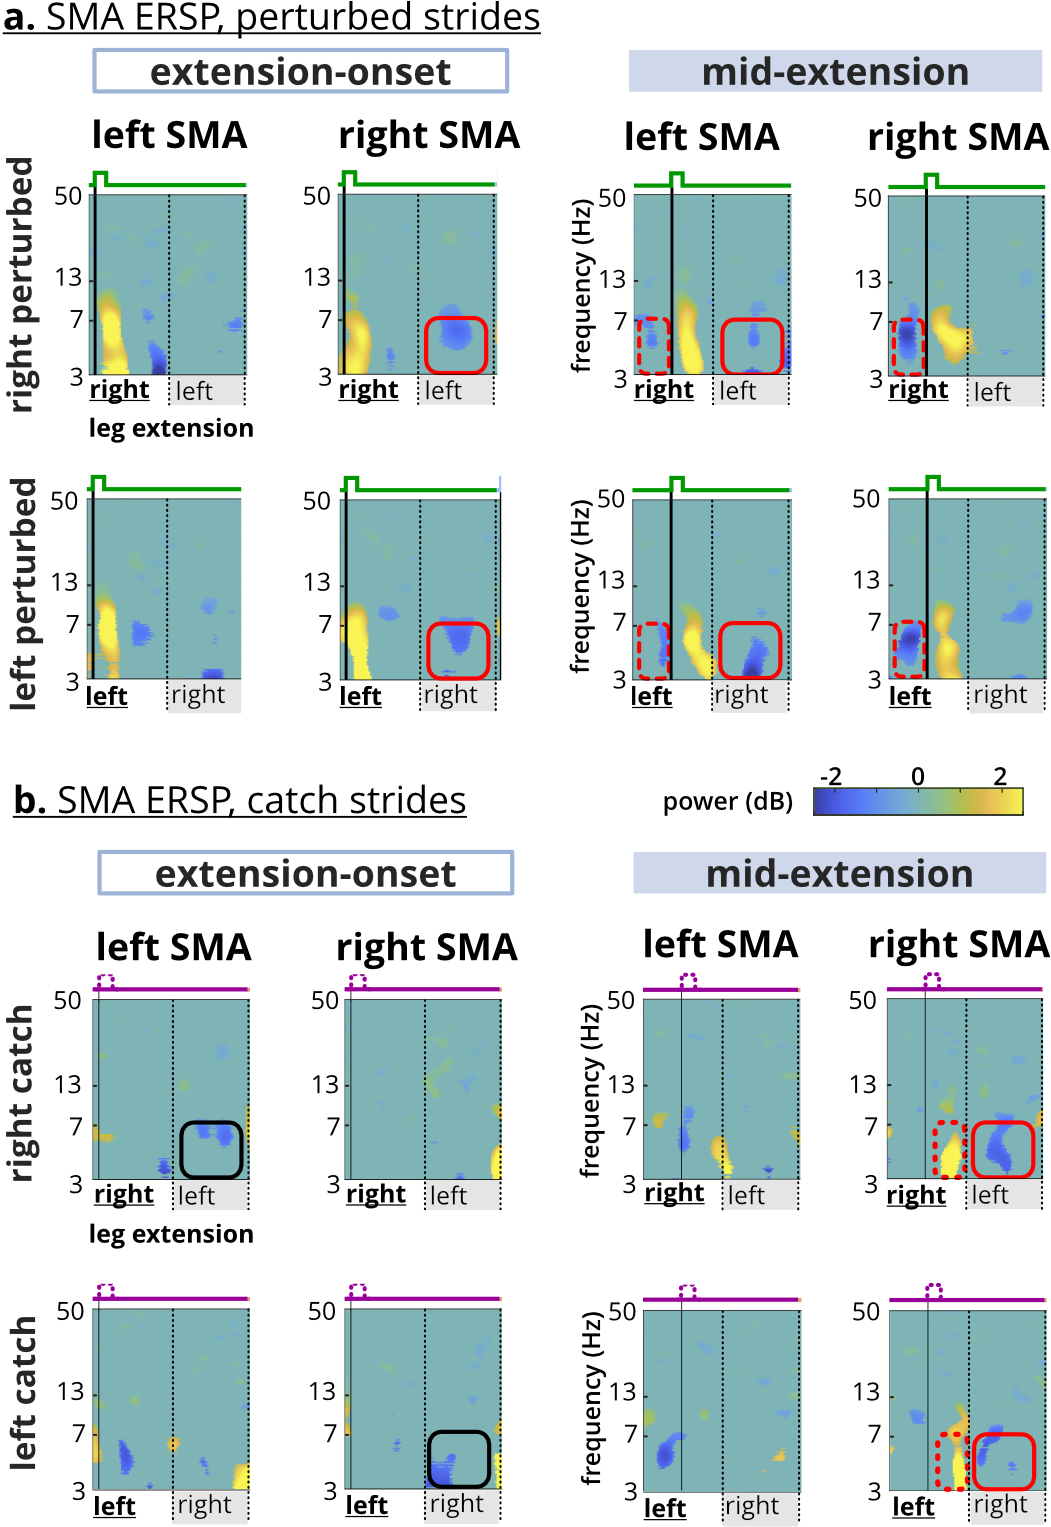
\includegraphics{figures/hyp4- lateraliztion.jpg}}
\caption{\textbf{Lateralization of the supplementary motor areas (SMAs).} \textbf{a.} Theta desynchronization in the perturbed recovery step occurred in the right SMA for extension-onset and in the left SMA for the mid-extension (red squares). Only mid-extension perturbations elicited theta desynchronization before the perturbation event in the both SMA clusters (red dashed rectangles). \textbf{b.} Mid-extension catch steps elicited theta synchronization right before the end of limb extension (red dashed rectangles). Recovery-step theta desynchronization occurred contralaterally during extension-onset, but only occurred in the right SMA during the mid-extension. Red rectangles indicate specialized lateralization and black rectangles indicate contralateral lateralization.}
\label{fig8}
\end{figure}

Perturbation timing significantly influenced anterior cingulate theta-band power fluctuations (Figure 6), suggesting that tuning perturbation features can modify and stimulate anterior cingulate activity. In this study, the theta-band average ERSP for extension-onset perturbations was greater than mid-extension perturbations. This difference may result from an additional intrinsic anterior cingulate theta synchronization that occurs during limb transitions in unperturbed gait, pedaling, and stepping \cite{Gramann2011-yj,Bulea2015-dv,Kline2014-pt,Enders2016-id}. While our results did not show significant anterior cingulate activity during pre and post-perturbations strides, our analyses and ICA was focused on identifying sources mostly present in perturbed stepping and accounted for the most information used in the analyses. Our results suggest that we can potentially tune the perturbations for enhanced or extended engagement of specific brain areas, such as the sustained anterior cingulate theta-band elicitation during the entire six minutes of left mid-extension perturbations.

We identified two close but distinct SMA clusters that exhibited specialized lateralization with both theta synchronization and desynchronization. We were able to identify distinct clusters in close proximity using our novel EEG noise rejection process that performs algorithmic parameter sweeping to estimate the most brain sources and an optimal k-means clustering algorithm to identify optimal cortical clusters (Figure 3). The left and right SMAs had clear differences in theta fluctuations (Figure 8), supporting that these SMA clusters were distinct and had specialized responses to the perturbations or motor errors. Theta synchronization occurred exclusively in the right SMA during mid-extension catch steps that had the largest temporal errors (\td250 ms), suggesting that despite the lack of a physical perturbation, the right motor area theta synchronization was still sensitive to a motor error. The right motor and premotor cortices have been linked with monitoring temporal aspects of motor tasks \cite{Mutha2014-ea,Wagner2016-nx}.

Interestingly, theta desynchronization occurred during the recovery step (i.e., the step following a perturbed step) in the right SMA during extension-onset perturbations and in the left SMA during mid-extension perturbations (Figure 8). Previous unperturbed gait studies showed significant theta desynchronization in sensorimotor cortices during mid-stance, but the significance of theta desynchronization specifically is not discussed \cite{Gramann2011-yj,Bradford2016-kp,Enders2016-id,Kline2016-ci}. A recent study demonstrated that theta synchronization and desynchronization corresponds to negative and positive deflections in event-related potentials (ERP) of motor cortex, respectively \cite{Nakagome2020-iv}. As such, ERP studies provide additional possible interpretations for observed theta synchronization and desynchronization in locomotor tasks. For example, a recent study on upper-limb visuomotor perturbations suggested that the presence (or absence) of negative and positive potentials during perturbations indicated different motor learning strategies \cite{Palidis2019-kg}, which aligns with our results.

Limitations of this study include not providing the subjects with explicit feedback about their errors, attributing cortical and motor adaptations to lower-limb extension, and not using a subject-specific head model for source estimation. We did not provide explicit feedback to avoid variations in the brain’s dynamics because of the additional cognitive load \cite{Kline2014-pt}. While recumbent stepping is a quadrupedal single degree of freedom task, we attributed the perturbations to the action of lower-limb extension, i.e., left mid-extension perturbation means the perturbation that is applied during left-leg mid-extension. Our stepping torque analysis (not reported here) and a previous study showed that subjects mainly used their lower limbs in response to higher power demand during recumbent stepping using the arms and legs \cite{Skinner2014-cl}. Finally, using a subject-specific electrical head model increases the accuracy of the source estimation process \cite{Akalin_Acar2013-rv}. However, combining the subject-specific head model with the step-wise cleaning approach was beyond our current computational capacity.

Mechanical perturbations are a robust way to elicit error-related cortical fluctuations and could be tuned to further enhance desired cortical activity. During a seated locomotor task, perturbations elicited anterior cingulate cortex activity, which decreased with more experience during the right-side perturbations. This supports that the anterior cingulate both monitors errors and learns from them \cite{Holroyd2002-fl}. The left and right SMA clusters demonstrated specialized lateralization, suggesting that tuning perturbation features such as timing can elicit more desired cortical activity. The uncoupled anterior cingulate activity with motor errors and specialized SMA fluctuations implicate that a cortical feedback may be crucial for closed-loop rehabilitation because motor changes may not adequately reflect cortical dynamics.

% \section{Acknowledgments}
% We would like to thank members of the Biomechanics, Rehabilitation, and Interdisciplinary Neuroscience (BRaIN) lab for their help with data collection and their constructive feedback. We also acknowledge the University of Central Florida \href{https://arcc.ist.ucf.edu}{Advanced Research Computing Center} for providing computational resources and support to run our novel step-wise noise rejection algorithm using 2500+ compute cores.

\bibliography{adapt_refs}
\bibliographystyle{ieeetr}
\end{document}
